% See exam.cls and examdoc.tex for the license information
\documentclass[12pt, answers]{exam}

\usepackage{amssymb}
\usepackage{makeidx}
\usepackage{amsmath}
\usepackage{graphicx}
\usepackage{caption}
\usepackage{tabulary}
\usepackage{color}
\usepackage{multicol}
\usepackage{multirow}
\usepackage{enumerate}
\usepackage{float}
\usepackage{colortbl}
\usepackage[table,xcdraw]{xcolor}
\usepackage{array}

\newcolumntype{C}[1]{>{\centering\let\newline\\\arraybackslash\hspace{0pt}}m{#1}}

\addpoints

% In case we're not using hyperref.sty:
\providecommand{\texorpdfstring}[2]{#1}
% The following can be used in \section commands
% without generating pdf warnings:
\newcommand{\bs}{\texorpdfstring{\char`\\}{}}

\makeindex

\newcommand{\indc}[1]{\index{#1@\texttt{\char`\\#1}}}
\newcommand{\indcsub}[2]{\index{#1@\texttt{\char`\\#1}!#2}}
\newcommand{\indcstart}[1]{\index{#1@\texttt{\char`\\#1}|(}}
\newcommand{\indcstop}[1]{\index{#1@\texttt{\char`\\#1}|)}}

\newcommand{\indt}[1]{\index{#1@\texttt{#1}}}
\newcommand{\indtsub}[2]{\index{#1@\texttt{#1}!#2}}
\newcommand{\indtstart}[1]{\index{#1@\texttt{#1}|(}}
\newcommand{\indtstop}[1]{\index{#1@\texttt{#1}|)}}

\extraheadheight{-.4in}

\pagestyle{headandfoot}
%\extraheadheight{.2 in}
\firstpageheader{}{}{}
\runningheader{}{}{}
\firstpagefooter{}{Progressing alignment}{Page \thepage\ of \numpages}
\firstpagefootrule
\runningfooter{}{Progressing alignment}{Page \thepage\ of \numpages}
\runningfootrule

%---------------------------------------------------------------------

\shadedsolutions
%\noprintanswers
\definecolor{SolutionColor}{rgb}{0.8,0.9,1}

\setcounter{section}{9}

\begin{document}

\section{Exercise solutions -- Progressing alignment}

%---------------------------------------------------------------------
\begin{questions}

%%% Question 1
\question \textbf{Linkage clustering method for progressive alignment}

Select two alignments from the three alignments, $\mathcal{A}^1={s^1}$, $\mathcal{A}^2={s^2, s^3}$, and $\mathcal{A}^3={s^4, s^5}$, for clustering.

\noindent
\begin{center}
Pairwise scores
\end{center}
\begin{table}[H]
\centering
\begin{tabular}{|c|c|c|c|c|c|}
\hline
   & $s^1$ & $s^2$ & $s^3$ & $s^4$ & $s^5$ \\ \hline
$s^1$ & -  & 2  & 3  & 1  & 6  \\ \hline
$s^2$ &    & -  & -  & 4  & 5  \\ \hline
$s^3$ &    &    & -  & 3  & 4  \\ \hline
$s^4$ &    &    &    & -  & -  \\ \hline
$s^5$ &    &    &    &    & -  \\ \hline
\end{tabular}
\end{table}

\begin{parts}

\vspace{0.1 in}

%% (a)
  \part Use the average linkage.

\begin{solution}[0.35 in]
$\mathcal{A}^2$ and $\mathcal{A}^3$: 
$S(\mathcal{A}^1, \mathcal{A}^2) = 2.5$, 
$S(\mathcal{A}^1,\mathcal{A}^3) = 3.5$, 
$S(\mathcal{A}^2, \mathcal{A}^3) = 4$
\end{solution}

%% (b)
  \part Use the maximum linkage.

\begin{solution}[0.35 in]
$\mathcal{A}^1$ and $\mathcal{A}^3$: 
$S(\mathcal{A}^1, \mathcal{A}^2) = 3 $, 
$S(\mathcal{A}^1,\mathcal{A}^3) = 6 $, 
$S(\mathcal{A}^2, \mathcal{A}^3) = 5$
\end{solution}

%% (c)
  \part Use the minimum linkage.

\begin{solution}[0.35 in]
$\mathcal{A}^2$ and $\mathcal{A}^3$: 
$S(\mathcal{A}^1, \mathcal{A}^2) = 2$, 
$S(\mathcal{A}^1,\mathcal{A}^3) = 1$, 
$S(\mathcal{A}^2, \mathcal{A}^3) = 3$
\end{solution}

\end{parts}


\newpage

%%% Question 2
\question \textbf{Linear progressive alignment}

Construct an MSA from seq1, seq2, seq3 and a phylogenetic tree by using the progressive alignment method specified below.

\begin{figure}[H]
      \centering
      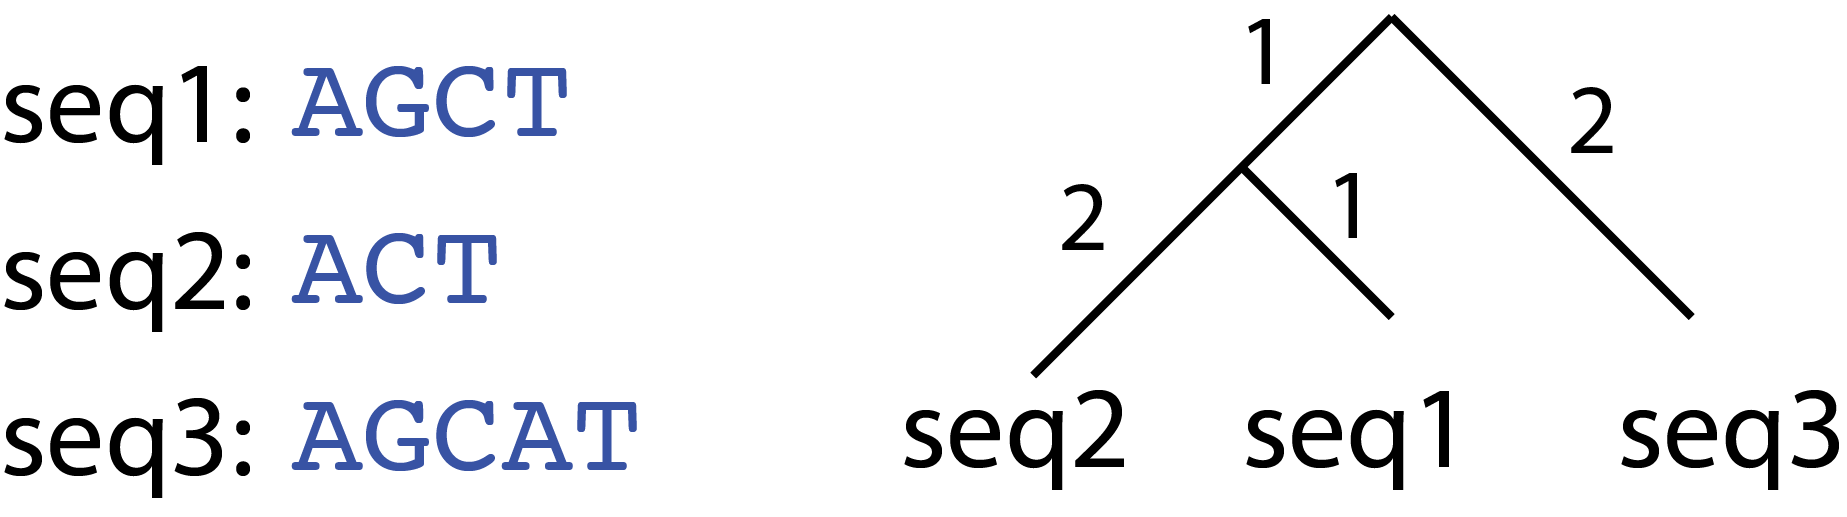
\includegraphics[width=0.4 \textwidth]{fig10/progressive_alignment_tree.png}
\end{figure}

\begin{itemize}
\item Clustering: Linear clustering
\item Aligning method: Pair-guided alignment
\item Aligning order: Use the specified tree 
\item Pairwise DP: Global alignment with linear gap penalty
\item DP scoring scheme: match (10), mismatch (-5), gap penalty (10)
\end{itemize}

\begin{parts}

\vspace{0.1 in}

%% (a)
  \part What is the aligning order that can be defined by the given tree? 

\begin{solution}[0.7 in]
\begin{verbatim}
1: Seq2 & Seq1
2: Seq1 & Seq3
\end{verbatim}
\end{solution}

%% (b)
  \part Solve the first pairwise alignment.

\begin{solution}[0.7 in]
\begin{verbatim}
Seq2: A-CT
Seq1: AGCT
\end{verbatim}
\end{solution}

%% (c)
  \part Solve the second pairwise alignment.

\begin{solution}[0.7 in]
\begin{verbatim}
Seq1: AGC-T
Seq3: AGCAT
\end{verbatim}
\end{solution}

%% (d)
  \part Find the optimal MSA by combining the first and the second alignments.

\begin{solution}[1.1 in]
\begin{verbatim}
Seq1: AGC-T
Seq2: A-C-T
Seq3: AGCAT
\end{verbatim}
\end{solution}

%% (e)
  \part What is the SP score of the optimal MSA?

\begin{solution}[1.7 in]
\begin{verbatim}
Seq1 & Seq2: 20
Seq1 & Seq3: 30
Seq2 & Seq3: 10

SP: 60
\end{verbatim}
\end{solution}

\end{parts}


\end{questions}
%---------------------------------------------------------------------
 
\end{document}

